\documentclass[
	a4paper,
	oneside,
	BCOR = 10mm,
	DIV = 12,
	12pt,
	headings = normal,
]{scrartcl}

%%% Length calculations
\usepackage{calc}
%%%

%%% Support for color
\usepackage{xcolor}
\definecolor{lightblue}{HTML}{03A9F4}
\definecolor{red}{HTML}{F44336}
%%%

%%% Including graphics
\usepackage{graphicx}
%%%

%%% Font selection
\usepackage{fontspec}

\setromanfont{STIX Two Text}[
	SmallCapsFeatures = {LetterSpace = 8},
]

\setsansfont{IBM Plex Sans}[
	Scale = MatchUppercase,
]

\setmonofont{IBM Plex Mono}[
	Scale = MatchUppercase,
]
%%%

%%% Math typesetting
\usepackage{amsmath}

\usepackage{unicode-math}
\setmathfont{STIX Two Math}

\usepackage{IEEEtrantools}
%%%

%%% List settings
\usepackage{enumitem}
\setlist[enumerate]{
	label*      = {\arabic*.},
	leftmargin  = *,
	labelindent = \parindent,
	topsep      = 1\baselineskip,
	parsep      = 0\baselineskip,
	itemsep     = 1\baselineskip,
	noitemsep, % override itemsep
}

\setlist[itemize]{
	label*      = {—},
	leftmargin  = *,
	labelindent = \parindent,
	topsep      = 1\baselineskip,
	parsep      = 0\baselineskip,
	itemsep     = 1\baselineskip,
	noitemsep, % override itemsep
}

\setlist[description]{
	font        = {\rmfamily\upshape\bfseries},
	topsep      = 1\baselineskip,
	parsep      = 0\baselineskip,
	itemsep     = 0\baselineskip,
}

%%%

%%% Structural elements typesetting
\setkomafont{pagenumber}{\rmfamily\upshape}
\setkomafont{disposition}{\rmfamily\bfseries}

% Sectioning
\RedeclareSectionCommand[
	beforeskip = -1\baselineskip,
	afterskip  = 1\baselineskip,
	font       = {\normalsize\bfseries\scshape},
]{section}

\RedeclareSectionCommand[
	beforeskip = -1\baselineskip,
	afterskip  = 1\baselineskip,
	font       = {\normalsize\bfseries\itshape},
]{subsection}

\RedeclareSectionCommand[
	beforeskip = -1\baselineskip,
	afterskip  = 1\baselineskip,
	font       = {\normalsize\bfseries},
]{subsubsection}

\RedeclareSectionCommand[
	beforeskip = -1\baselineskip,
	afterskip  = -0.5em,
	font       = {\normalsize\mdseries\scshape\addfontfeatures{Letters = {UppercaseSmallCaps}}},
]{paragraph}
%%%

%%% Typographic enhancements
\usepackage{microtype}
%%%

%%% Language-specific settings
\usepackage{polyglossia}
\setmainlanguage{ukrainian}
\setotherlanguages{english}
%%%

%%% Captions
\usepackage{caption}
\usepackage{subcaption}

%\DeclareCaptionLabelFormat{closing}{#2)}
%\captionsetup[subtable]{labelformat = closing}

%\captionsetup[subfigure]{labelformat = closing}

\captionsetup[table]{
	aboveskip = 0\baselineskip,
	belowskip = 0\baselineskip,
}

\captionsetup[figure]{
	aboveskip = 1\baselineskip,
	belowskip = 0\baselineskip,
}

\captionsetup[subfigure]{
	labelformat = simple,
	labelformat = brace,
}
%%%

%%% Hyphenated ragged typesetting
\usepackage{ragged2e}
%%%

%%% Table typesetting
\usepackage{booktabs}
\usepackage{longtable}

\usepackage{multirow}

\usepackage{array}
\newcolumntype{v}[1]{>{\RaggedRight\arraybackslash\hspace{0pt}}p{#1}}
\newcolumntype{b}[1]{>{\Centering\arraybackslash\hspace{0pt}}p{#1}}
\newcolumntype{n}[1]{>{\RaggedLeft\arraybackslash\hspace{0pt}}p{#1}}
%%%

%%% Drawing
\usepackage{tikz}
\usepackage{tikzscale}
\usetikzlibrary{positioning}
\usetikzlibrary{arrows.meta} % Stealth arrow tips
%%%

%%% SI units typesetting
\usepackage{siunitx}
\sisetup{
	output-decimal-marker = {,},
	exponent-product      = {\cdot},
	inter-unit-product    = \ensuremath{{} \cdot {}},
	per-mode              = symbol,
}
%%%

%%% Framing code listings
\usepackage{tcolorbox}
\tcbuselibrary{breakable}
\tcbuselibrary{minted}
\tcbuselibrary{skins}

\newtcblisting[
	auto counter, 
	list inside, 
	number within = section,
]{listingpython}[3][]{%
	minted language = python,
	minted style    = bw,
	minted options  = {
		linenos,
		tabsize = 4,
		breaklines,
		% breakanywhere,
		fontsize = \footnotesize,
		autogobble
	},
	%
	% empty,
	sharp corners,
	colframe         = black,
	colback          = black!0,
	leftrule         = 0em,
	rightrule        = 0em,
	toprule          = 1pt, % orig = 0pt
	bottomrule       = 1pt, % orig = 0pt
	titlerule        = 0.5pt,
	colbacktitle     = black!0,
	coltitle         = black,
	toptitle         = 0.3em,
	bottomtitle      = 0.1em,
	borderline north = {1pt}{0pt}{black},
	borderline south = {1pt}{0pt}{black},
	before skip      = \intextsep,
	after  skip      = \intextsep,
	title            = {Лістинг \thetcbcounter: #2},
	list entry       = {\protect\numberline{\thetcbcounter}#2},
	left = 0em,
	right = 0em,
	%
	listing only,
	breakable,
	%
	label = {#3},
	%
	#1
}

\newtcbinputlisting[auto counter, list inside, number within = section]{\inputpython}[4][]{%
	minted language = python,
	minted style    = bw,
	minted options  = {
		linenos,
		tabsize = 4,
		breaklines,
		breakbytokenanywhere,
		fontsize = \footnotesize,
	},
	%
	% empty,
	sharp corners,
	colframe         = black,
	colback          = black!0,
	leftrule         = 0em,
	rightrule        = 0em,
	toprule          = 0pt, % orig = 0pt
	bottomrule       = 0pt, % orig = 0pt
	titlerule        = 0.5pt,
	colbacktitle     = black!0,
	coltitle         = black,
	toptitle         = 0.3em,
	bottomtitle      = 0.1em,
	borderline north = {1pt}{0pt}{black},
	borderline south = {1pt}{0pt}{black},
	before skip      = \intextsep,
	after  skip      = \intextsep,
	title            = {Лістинг \thetcbcounter: #3},
	list entry       = {\protect\numberline{\thetcbcounter}#3},
	left = 0em,
	right = 0em,
	%
	listing file={#2},
	listing only,
	breakable,
	%
	label = {#4},
	%
	#1
}

% Customize minted
\usepackage{minted}
\setmintedinline{
	style = bw,
	breaklines,
}

% Customize minted line numbers
\renewcommand{\theFancyVerbLine}{\ttfamily\scriptsize\arabic{FancyVerbLine}}

%%%

%%% Links and hyperreferences
\usepackage{hyperref}
\hypersetup{
	bookmarksnumbered = true,
	colorlinks      = false,
	linkbordercolor = red,
	urlbordercolor  = lightblue,
	pdfborderstyle  = {/S/U/W 1.5},
}
%%%

%%% Length adjustments
% Set baselineskip, default is 14.5 pt
\linespread{1.068966} % ~15.5 pt
\setlength{\emergencystretch}{1em}
\setlength{\parindent}{1.5em}
\newlength{\gridunitwidth}
\setlength{\gridunitwidth}{\textwidth / 12}
%%%

%%% Custom commands
\newcommand{\allcaps}[1]{{\addfontfeatures{LetterSpace = 8, Kerning = Off}#1}}
\newcommand{\filename}[1]{\texttt{#1}}
\newcommand{\progname}[1]{\texttt{#1}}
\newcommand{\modulename}[1]{\texttt{#1}}
%%%

%%% Custom math commands
\newcommand{\longvar}[1]{\mathit{#1}}
%%%

\begin{document}

\begin{titlepage}
		\begin{center}
			Міністерство освіти і науки України\\
			Національний авіаційний університет\\
			Навчально-науковий інститут комп'ютерних інформаційних технологій\\
			Кафедра комп'ютеризованих систем управління

			\vspace{\fill}
				Лабораторна робота №2\\
				з~дисципліни «Імітаційне моделювання»\\
				на~тему «Моделювання випаадкових подій»\\

			\vspace{\fill}

			\begin{flushright}
				Виконав:\\
				студент \allcaps{ННІКІТ}\\
				групи СП-325\\
				Клокун В.\,Д.\\
				Перевірила:\\
				Марченко Н.\,Б.
			\end{flushright}

			Київ 2019
		\end{center}
	\end{titlepage}

	\section{Мета роботи}
		Ознайомитись з~алгоритмами моделювання результатів випробувань випадкових подій; побудувати імітаційну модель функціонування системи протягом деякого часу.

	\section{Хід роботи}
		Для виконання роботи задані такі завдання:
		\begin{enumerate}
			\item Задано задачу 1 загального виду: система $S_1$ працює протягом деякого часу~$t$ і~складається з~$m$ підсистем, кожна з яких незалежно одна від одної може вийти з ладу впродовж деякого часу~$t$. Ймовірність безвідмовної роботи кожної підсистеми визначається так: $P(n_i) = p_i$. Побудувати імітаційну модель функціонування системи~$S_1$ протягом часу~$t$, використовуючи генератор псевдовипадкових чисел на інтервалі~$(0; 1)$. Усі дані вводяться користувачем.
			\item Задано задачу 2 загального виду: система~$S_2$ складається з~2~підсистем, які пов'язані між собою. Ймовірність безвідмовної роботи підсистеми~$n_1$ протягом часу~$t$ є~$P(n_1) = p_1$. Ймовірність роботи другої підсистеми~$n_2$ така: $P(n_i) = p_i$. Побудувати імітаційну модель функціонування системи~$S_2$ протягом часу~$t$, використовуючи генератор псевдовипадкових чисел на інтервалі~$(0; 1)$.
		\end{enumerate}

		Під час виконання роботи були розроблені імітаційні моделі для виконання поставлених завдань і реалізовані у вигляді відповідного програмного засобу (ліст.~\ref{lst:full-solution}). Реалізований програмний засіб був запущений на моделювання і надавав стабільний і~очікуваний результат~(рис.~\ref{fig:res}).

		\begin{figure}[!htbp]
			\centering
			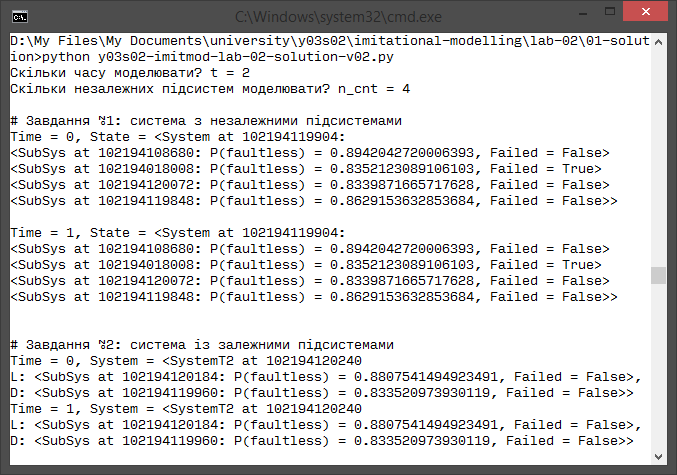
\includegraphics[height = 10\baselineskip]{./assets/y03s02-imitmod-lab-02-p00.png}
			\caption{Результат роботи реалізованого програмного засобу}
			\label{fig:res}
		\end{figure}

		\section{Висновок}
			Виконуючи дану лабораторну роботу, ми ознайомились з~алгоритмами моделювання результатів випробувань випадкових подій; побудували імітаційну модель функціонування системи протягом деякого часу.

		\appendix
		\section{Повний початковий код програмної реалізації}
		\label{sec:full-listing}
			\begin{listingpython}[toprule = 0pt, bottomrule = 0pt]{Повний початковий код програмної реалізації}{lst:full-solution}
#!/usr/bin/env python3

import random  # random.random(), random.uniform()


class Subsystem(object):
    """ Subsystem --- основний клас-підсистема для завдань №№1, 2
    """
    def __init__(self, p_faultless=0.0, failed=False):
        self._p_faultless = p_faultless
        self._failed = failed

    def __str__(self):
        """ Визначає представлення об'єкту даного класу у вигляді рядка """
        s = (
            '<SubSys at {}: P(faultless) = {}, Failed = {}>'
            .format(id(self), self.p_faultless, self.failed)
        )

        return s

    @property
    def p_faultless(self):
        """ Ймовірність безвідмовної роботи """
        return self._p_faultless

    @p_faultless.setter
    def p_faultless(self, value):
        """ Дозволяє задати значення ймовірності безвідмовної роботи """
        self._p_faultless = value

    @property
    def failed(self):
        """ Статус, що система непрацездатна """
        return self._failed

    @failed.setter
    def failed(self, value):
        self._failed = value

    def _fail(self):
        """ Робить систему непрацездатною """
        self.failed = True

    def run(self):
        """ Запускає систему у даний момент часу.

        Якщо система вже непрацездатна, завершити роботу і повернути статус
        непрацездатності. Інакше перевірити, чи зламається система у даний
        момент часу і також повернути статус непрацездатності.
        """
        if self.failed:
            return self.failed
        elif random.random() > self.p_faultless:
            self._fail()

        return self.failed


class SystemType1(object):
    """ Система з незалежними підсистемами """
    def __init__(self, subsystems=None):
        self._subsystems = subsystems

    def __str__(self):
        s = ''
        subsys_list = [str(subsys) for subsys in self.subsystems]
        s = '\n'.join(subsys_list)
        s = (
            '<System at {}:\n'
            '{}>'.format(id(self), s)
        )

        return s

    @property
    def subsystems(self):
        return self._subsystems

    def add_subsystem(self, subsystem):
        self.subsystems.append(subsystem)

    def run(self, time=1):
        for t in range(time):
            for s in self.subsystems:
                s.run()

            print('Time = {}, State = {}\n'.format(t, str(self)))

    def get_state(self):
        state = ''
        for s in self.subsystems:
            state += ''.format(str(s))

        return state


class SubsystemDependant(Subsystem):
    """ Залежна система для завдання №2.

    Успадковує та розширює незалежну підсистему
    """
    def __init__(self, p_faultless=0.0, p_faultless_leader_failed=0.0,
                 failed=False):
        self._p_faultless = p_faultless
        self._failed = failed

        self._p_faultless_leader_failed = p_faultless_leader_failed

    @property
    def p_faultless_leader_failed(self):
        return self._p_faultless_leader_failed

    @p_faultless_leader_failed.setter
    def p_faultless_leader_failed(self, value):
        self._p_faultless_leader_failed = value

    def run_leader_faulty(self):
        """ Метод, який описує процес роботи підсистеми у системі, де її головна
        підсистема непрацездатна
        """
        if self.failed:
            return self.failed
        elif random.random() > self.p_faultless_leader_failed:
            self._fail()

        return self.failed


class SystemType2(object):
    """ Система із головною і залежною підсистемою для
    завдання 2
    """
    def __init__(self, leader, dependant):
        """ Конструктор
        """
        self.subsys_leader = leader
        self.subsys_dependant = dependant

    def __str__(self):
        """ Визначає, як об'єкт даного класу виглядатиме у вигляді рядка
        """
        s = (
            '<SystemT2 at {}\n'
            'L: {},\n'
            'D: {}>'
            .format(id(self), self.subsys_leader, self.subsys_dependant)
        )
        return s

    def run_once(self):
        """ Запускає систему в один момент часу """
        # Запустити незалежну підсистему
        self.subsys_leader.run()
        # Якщо незалежна підсистема не зламалась, запустити залежну у звичайному
        # режимі
        if not self.subsys_leader.failed:
            self.subsys_dependant.run()
        # Інакше --- у режимі зламаної головної підсистеми
        else:
            print('Leader failed.')
            self.subsys_dependant.run_leader_faulty()

    def run(self, time=1):
        for t in range(time):
            self.run_once()
            print(
                'Time = {}, System = {}'
                .format(t, str(self))
            )


def main():
    runtime = int(input('Скільки часу моделювати? t = '))
    n_cnt = int(input('Скільки незалежних підсистем моделювати? n_cnt = '))
    # Завдання 1
    print('\n# Завдання №1: система з незалежними підсистемами')

    # Створюємо незалежні підсистеми
    subsystems = [
        Subsystem(p_faultless=random.uniform(0.8, 0.9))
        for _ in range(n_cnt)
    ]
    # Створюємо систему з незалежних підсистем
    system1 = SystemType1(subsystems)
    # Запускаємо її
    system1.run(time=runtime)

    # Завдання 2
    print('\n# Завдання №2: система із залежними підсистемами')

    # Створюємо систему з головною і залежною підсистемою
    system2 = SystemType2(
        # Головна
        leader=Subsystem(p_faultless=random.uniform(0.8, 0.9)),
        # Залежна
        dependant=SubsystemDependant(
            # Ймовірність безвідмовної роботи, коли головна система справна
            p_faultless=random.uniform(0.8, 0.9),
            # Ймовірність безвідмовної роботи, коли головна система несправна
            p_faultless_leader_failed=random.uniform(0.6, 0.8)
        ),
    )
    # Запускаємо її
    system2.run(time=runtime)


if __name__ == '__main__':
    main()
			\end{listingpython}

\end{document}

